\section{Ejercicio 8}


\subsection{Desarrollo}
Similar  a lo visto en el ejercicio 8, tendremos que programar la estructura de un scheduler de Round-Robin. La diferencia es que en este caso en vez de tener una cola única 
que vaya guardando todos los procesos, cada core tendrá su propia cola de procesos. Para resolver esto utilizaremos una estructura para representar el core que nos dará la 
siguiente información: un entero pidActual, un entero cpu$\_$quantum, un entero quantum$\_$restantes, su cola de pids enEspera, un vector pid$\_$bloqueados que indica cuales están en ese estado.

Después tenemos la cantidad de cores y el quantum de los mismos. Por último necesitamos agrupar las estructuras core que tenemos. Para esto usamos simplemente un vector 
(nucleos).

La función load lo que hace es buscar cual de los cores tiene menor cantidad de procesos(suma los bloqueados, los de enEspera y el de pidActual, si no es IDLE). Una vez 
encontrado, lo encola en el enEspera del core.

unblock lo que hace es buscar cual es el core donde se encuentra el pid que se desea bloquear, una vez encontrado lo quita de pid$\_$bloqueados y lo pone en enEspera.

Por último tenemos la función tick. El código es equivalente al del ejercicio 4.


\subsection{Experimentación}
Según lo pedido debemos mencionar un caso donde la migración de núcleos sea beneficiosa y otro donde no. Para lo segundo, usaremos dos core y cuatro tareas que irán apareciendo
en este orden: la más costosa,  la menos costosa, la segunda más costosa y la segunda menos costosa. Usaremos, en los dos cores, un quantum de 5(para todos) y nos queda lo siguiente:

\begin{figure}[H]
  \centering
    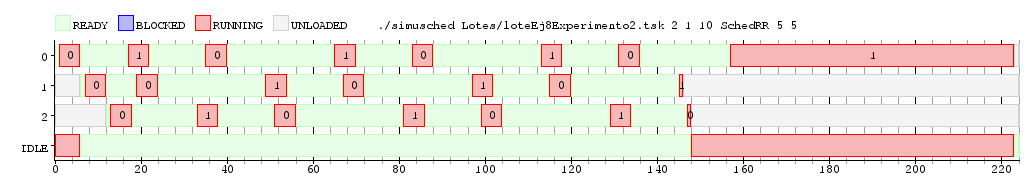
\includegraphics[width=1.1\textwidth]{imagenes/Ej8Experimento3.png}
  \caption{loteEj8Experimento1.tsk con RR}
\end{figure}

\begin{figure}[H]
  \centering
    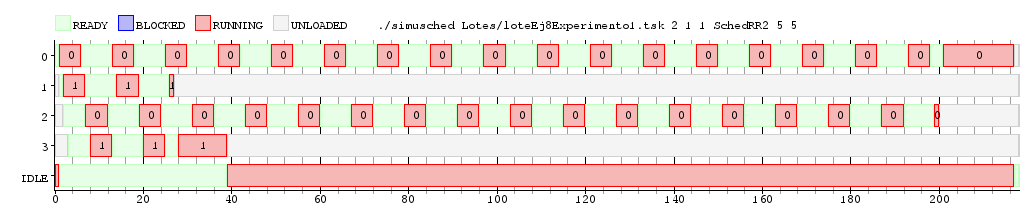
\includegraphics[width=1.1\textwidth]{imagenes/Ej8Experimento1.png}
  \caption{loteEj8Experimento1.tsk con RR2}
\end{figure}

Para el caso en el que sea beneficiosa vamos a usar el mismo lote de tareas, pero las cambiaremos de orden para que sean así: 
la más costosa, la segunda más costosa, la menos costosa y la segunda menos costosa. Nos queda lo siguiente:

\begin{figure}[H]
  \centering
    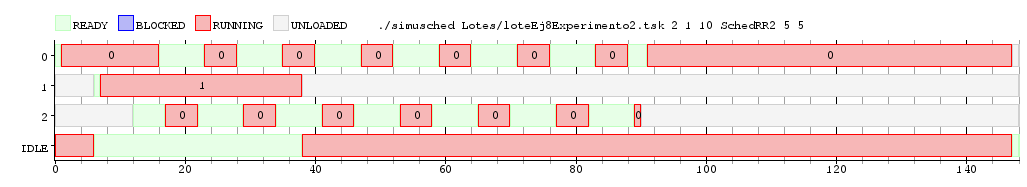
\includegraphics[width=1.1\textwidth]{imagenes/Ej8Experimento4.png}
  \caption{loteEj8Experimento2.tsk con RR}
\end{figure}

\begin{figure}[H]
  \centering
    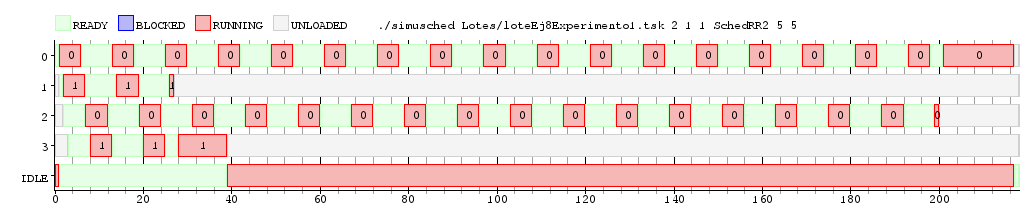
\includegraphics[width=1.1\textwidth]{imagenes/Ej8Experimento2.png}
  \caption{loteEj8Experimento2.tsk con RR2}
\end{figure}

Podemos ver que efectivamente el primer caso se tarda más en completar los procesos con RR2 que con RR. Esto se debe a que el orden que le dimos a las tareas hace que el primer
procesador se le asigne las tareas más largas y costosas, mientras que el segundo tiene las más cortas. En ese sentido se muestra como la mayor parte del trabajo recae en uno de ellos
mientras que el otro termina y queda en ready mucho más rápido. Para el segundo experimento, al cambiar el orden podemos apreciar que los dos procesadores tienen una tarea muy costosa y otra no tanto. Efectivamente termina más rápido que el de RR común ya que el trabajo se distribuye de forma más justa. Para el que posee migración de procesos, obserbamos que terminan al mismo tiempo para los dos casos. Esto se debe a que en realidad el orden de estas tareas, que es lo que cambia, no afecta demasiado a la ejecución como tal a diferencia del otro sched.

